% !TeX spellcheck = es_ES
%%%%%%%%%%%%%%%%%%%%%%%%%%%%%%%%%%%%%%%%%
% Stylish Article
% LaTeX Template
% Version 2.1 (1/10/15)
%
% This template has been downloaded from:
% http://www.LaTeXTemplates.com
%
% Original author:
% Mathias Legrand (legrand.mathias@gmail.com) 
% With extensive modifications by:
% Vel (vel@latextemplates.com)
% Final ACS by:
% Juan Barbosa
% License:
% CC BY-NC-SA 3.0 (http://creativecommons.org/licenses/by-nc-sa/3.0/)
%
%%%%%%%%%%%%%%%%%%%%%%%%%%%%%%%%%%%%%%%%%
\documentclass[fleqn,10pt]{SelfArx}
%\usepackage[superscript]{cite}
\usepackage{wrapfig}
\usepackage{multirow}
%----------------------------------------------------------------------------------------
%	ARTICLE INFORMATION
%----------------------------------------------------------------------------------------

\JournalInfo{Laboratorio de Bioquímica, 07/02/2019} % Journal information
\Archive{ }

\PaperTitle{Aislamiento y determinación de ácidos nucleicos} %
%\Keywords{Keyword1 --- Keyword2 --- Keyword3} % Keywords - if you don't want any simply remove all the text between the curly brackets
%\newcommand{\keywordname}{Keywords} % Defines the keywords heading name

%----------------------------------------------------------------------------------------
%	ABSTRACT
%----------------------------------------------------------------------------------------

\Abstract{
In this practice we determine the presence of nucleic acids in biological samples: vegetable, fungal and bacterial, using UV-vis spectroscopy. The purity of the DNA for the \textit{E. coli} and \textit{S. aureus} bacteria samples was discussed taking into account the absorptions at 230, 260 and 280 nm, finding a correlation between the absorbance of the aromatic amino acids and the peptide bonds for the first two, and a small increase in the expected value in the case of the \textit{S. cerevisiae}. Likewise, the steps involved in the isolation of nucleic acids were discussed
}

%----------------------------------------------------------------------------------------

\begin{document}

\flushbottom % Makes all text pages the same height

\maketitle % Print the title and abstract box
%\tableofcontents % Print the contents section

\thispagestyle{empty} % Removes page numbering from the first page



%----------------------------------------------------------------------------------------
%	ARTICLE CONTENTS
%----------------------------------------------------------------------------------------

\section*{Introducci\'on} % The \section*{} command stops section numbering
%------------------------------------------------
	El ácido desoxirribonucleico (ADN) es la molécula que contiene y transmite la información genética de los organismos. Está formado por dos cadenas complementarias de nucleótidos que se enrollan entre sí formando una doble hélice que se mantiene unida por enlaces de hidrógeno entre bases complementarias (\autoref{fig2}). Los cuatro nucleótidos que forman el ADN contienen las bases adenina (A), guanina (G), citosina (C) y timina (T). En esta estructura se encuentran especificadas las secuencias de aminoácidos de todas las proteínas y las secuencias de nucleótidos de todas las moléculas de ARN. Las únicas funciones conocidas del ADN son el almacenamiento y la transmisión de la información biológica \cite{dahm2005friedrich, nelson2008lehninger, watson1953molecular}.
	\begin{figure}[h]
		\centering
		
\includegraphics[width=\linewidth]{dna}
		\caption{Estructura doble hélice de ADN}
		\label{fig2}
	\end{figure}
	
	El ADN fue aislado y caracterizado por primera vez por Friedrich Miescher en 1868. A esta sustancia que contenía fosforo la denominó “nucleína”. Posteriormente, en 1930 Phoebus Levende en colaboración con su maestro, demostraron que el solido aislado por Miescher estaba compuesto por 4 bases nitrogenadas, un grupo fosfato y un azúcar. Pero no fue hasta 1953 cuando James Watson, Francis Crick y Maurice Wilkins descubrieron, mediante difracción de rayos X, la estructura de doble hélice que la caracteriza \cite{nelson2008lehninger, watson1953molecular, maddox2003double}.
	
	Hasta este momento no había pruebas claras de que el ADN era el material genético, hasta que Avery y colaboradores encontraron que el ADN extraído de una cepa virulenta (causante de enfermedad) de la bacteria Streptococciís pneumoniae, e inyectado a una cepa no virulenta de la misma bacteria, era capaz de transformar una cepa no virulenta en una virulenta. Esto permitió llegar a la conclusión de que el ADN extraído de la cepa virulenta transportaba la información genética de la virulencia \cite{dahm2005friedrich}.
	
	En la célula se encuentran varias clases de ARN, los cuales, cubren una amplia variedad de funciones. Por ejemplo, los ARN ribosómicos (rARN) son componentes de los ribosomas, los cuales son complejos que llevan a cabo la síntesis de proteínas. Por otra parte, los ARN mensajeros (mARN) actúan de intermediarios transportando la información desde un gen o unos pocos genes hasta el ribosoma, donde se sintetizan las proteínas. Por ultimo los ARN de transferencia (tARN) son moléculas adaptadoras que traducen la información contenida en el mARN a secuencias específicas de aminoácidos \cite{nelson2008lehninger, watson1953molecular, maddox2003double}.
	
	Los ácidos nucleicos, el ADN y ARN reciben su nombre del hecho de ser moléculas con características acídicas y de haberse localizado inicialmente en el núcleo celular, aunque ahora se sabe que también se encuentran en la mitocondria. Para su estudio los ácidos nucleicos deben aislarse del resto de los componentes celulares, como lípidos y proteínas, los cuales, son más abundantes que los ácidos nucleicos. Así mismo, dependiendo del estudio de interés, debe aislarse de preferencia el ADN o ARN; así, para estudios de niveles de expresión génica se extraerá ARN, mientras que para la búsqueda de modificaciones o alteraciones génicas, el ADN \cite{dahm2005friedrich, watson1953molecular, maddox2003double}.
	
	El análisis de este tipo de compuestos se puede realizar mediante espectrofotometría UV-VIS, esto debido a que las interacciones próximas del apilamiento de las bases de los ácidos nucleicos dan lugar a una disminución de la absorción de la luz UV, en relación con la absorción de una disolución de nucleótidos libres de la misma concentración. Este fenómeno se denomina efecto hipocrómico. La desnaturalización de un ácido nucleico de doble cadena produce el efecto contrario, es decir, un incremento de la absorción, denominado efecto hipercrómico. La transición del ADN de cadena doble a la forma de cadena sencilla desnaturalizado puede seguirse, por tanto, midiendo la absorción de luz UV de 260 nm \cite{nelson2008lehninger}.
	\newpage
	
	Por lo cual, en el siguiente informe se realizó el aislamiento de ARN de levadura seca comercial, ADN de fresa y ADN genómico de bacterias \textit{Escherichia coli} y \textit{Staphylococcus aureu}. Por ultimo se realizó un análisis de estos ácidos nucleicos mediante espectrofotometría UV-VIS tomando un espectro de 200 nm a 300 nm de cada una de las muestras obtenidas.
	
\section{Secci\'on experimental}
	\subsection{Materiales}
	Para esta practica se utilizaron muestras comerciales de levadura seca, fresas, piña, detergente lavavajillas y filtros de café. Así mismo se utilizo una centrifuga ThermoScientific SL 8R.
	
	\subsection{Aislamiento de ARN de levadura}
	Para comenzar se suspendieron 2.5 g de levadura seca en 10 mL de agua tipo 1 a 37 $^\circ$C durante 15 minutos. Posteriormente se prepararon 10 mL de una solución saturada de fenol (8 g de fenol para 100 mL a 20 $^\circ$C), se añadió esta solución a la suspensión de levadura y se agitó durante 30 minutos. Transcurrido este tiempo se depositaron los 20 mL de mezcla en un tubo falcon de 50 mL y se llevó a centrifugación a 3000 rpm durante 15 minutos. Después de esto se recupero la capa superior acuosa y se llevó a centrifugación nuevamente, pero esta vez a 4500 rpm, durante 5 minutos para separar la proteína desnaturalizada. Posteriormente se tomó el sobrenadante y se agregó acetato de potasio hasta obtener una concentración final de 20 mg/mL, luego, se precipito el ARN añadiendo 10 mL de etanol frío y se dejo enfriar la mezcla en un baño de hielo durante 1 hora. Al terminar este tiempo se volvió a centrifugar la mezcla durante 5 minutos. Se lavó el ARN precipitado con una mezcla etanol agua, luego con éter etílico y se seco con una suave corriente de aire. Por último, se disolvió el ARN en la mínima cantidad de agua tipo 1 con ayuda de calentamiento a 37 $^\circ$C.
	
	\subsection{Aislamiento de ADN de fresa}
	Se realizo una mezcla de 1.5mL de detergente lavavajillas, 0.5 g de cloruro de sodio, 20 mL de agua tipo 1 y una fresa cortada en trozos pequeños dentro de una licuadora y se llevó a máxima velocidad durante 30 segundos. Después de esto se filtro la mezcla obtenida con un filtro de café. Por otra parte, se preparó zumo de piña licuando pedazos de piña sin agua y sin cascara y se filtro con un filtro de café. Posteriormente se mezcló en un beaker de 50 mL la solución de fresa filtrada anteriormente junto a 1.5 mL del zumo de piña y se agito hasta lograr homogeneizar la solución. Se añadieron 20 mL de etanol muy frío por las paredes del beaker permitiendo la formación de una capa sobre el filtrado y se dejo reposar hasta que se formó una zona turbia entre las dos fases. Después de esto se introdujo una pipeta Pasteur en la zona turbia y se extrajeron las marañas de fibras blancas de ADN. Por último, se lavó el ADN precipitado con una mezcla agua-etanol, con éter etílico, se secó suavemente bajo una corriente de aire. Finalmente se disolvió en la mínima cantidad de agua tipo 1 con ayuda de calentamiento a 37 $^\circ$C.
	
	\subsection{Aislamiento de ADN genómico de bacterias}
	Se tomaron 5 mL de un \textit{overnight} de \textit{Escherichia coli} y \textit{Staphylococcus aureus} y se transfirieron a tubos falcon de 15 mL cerca al mechero. Posteriormente se dejaron las muestras en un baño de maría en ebullición por 20 minutos y transcurrido este tiempo se dejaron en un baño de hielo por 5 minutos. Por ultimo se llevo a centrifugar a 4500 rpm durante 5 minutos y se tomo el sobrenadante con ayuda de una pipeta Pasteur.
	
	\subsection{Análisis de ácidos nucleicos}
	Se tomó un espectro UV-VIS de 200 nm a 300 nm de cada una de las muestras obtenidas. Se registraron las absorbancias a 230 , 260 y 280 nm.
	
\section{Resultados y Discusi\'on}
	\subsection{Aislamiento del ARN de levadura}
		Al disolver la levadura comercial en agua a una temperatura de 37 $^\circ$C se busca activar el metabolismo del hongo, para que esto pueda suceda es necesario que el organismo produzca ARN con el fin de iniciar la producci\'on de prote\'inas. En este sentido el control de la temperatura debe ser estricto, dado que cambios aumentos abruptos en esta, pueden llevar a que el organismo muera y cese su producci\'on del ARN que posteriormente ser\'a cuantificado.
		
		La adici\'on de fenol permite extraer los \'acidos nucleicos de la levadura dada la polaridad del mismo. Los \'acidos nucleicos debido a sus grupos fosfatos, constituyen mol\'eculas polares, las cuales se disuelven mejor en agua que en fenol. El proceso contrario sucede con las prote\'inas, las cuales tender\'an a estar en la fase org\'anica. La centrifugaci\'on de esta mezcla permite realizar la separaci\'on de fases, en donde en la fase acuosa se obtienen mayormente \'acidos nucleicos y prote\'inas desnaturalizadas. La siguiente centrifugaci\'on permite aislar los \'acidos nucleicos de las prote\'inas desnaturalizadas.
		
		Finalmente, y con el objetivo de precipitar los \'acidos nucleicos se adiciona acetato de potasio y etanol, los cuales promueven la formaci\'on de enlaces entre los aniones de los grupos fosfatos de los \'acidos nucleicos, y el ion potasio, con lo cual se neutraliza la mol\'ecula, ocasionando su precipitaci\'on.
		
	\begin{figure*}[h]
		\centering
		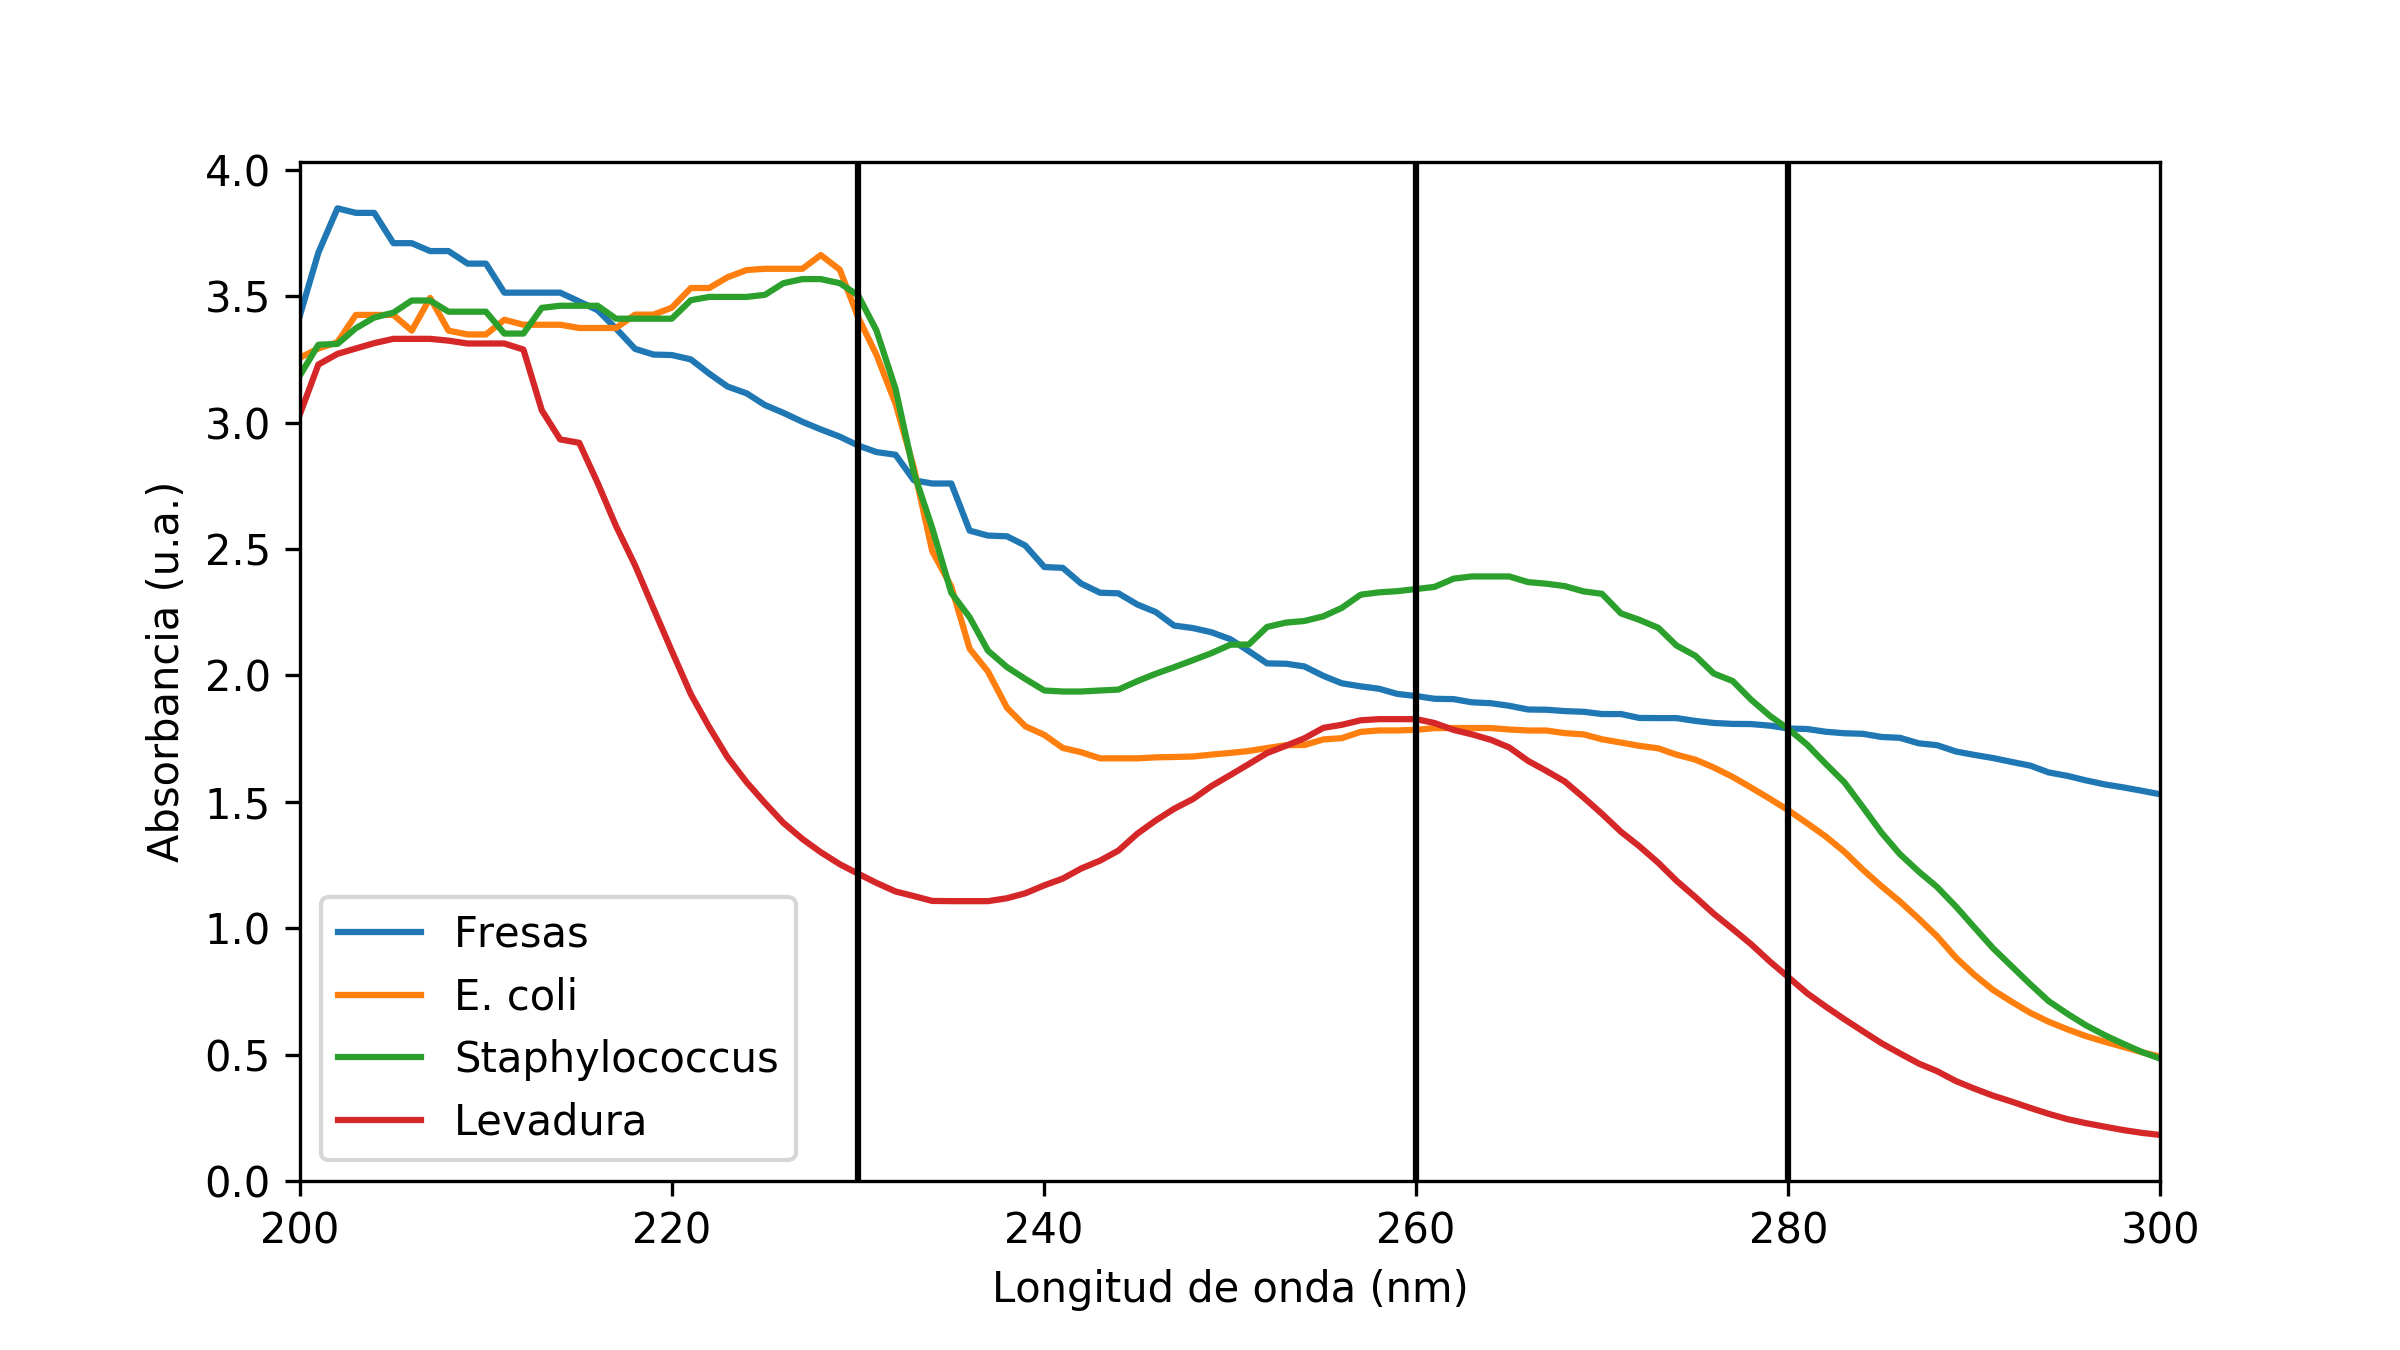
\includegraphics[width=\linewidth]{plots}
		\caption{Absorbancias obtenidas para las distintas muestras en funci\'on de la longitud de onda.}
		\label{fig}
	\end{figure*}		
	
	\subsection{Aislamiento del ADN de fresa}
		Para extraer el ADN de la \textit{F. ananassa}, se hace uso de detergente, el cual tiene como objetivo disolver las membranas de las células, en un proceso conocido como lisis \cite{virgili2006genoma, puerta2005practicas}. Al disolver las proteínas se interrumpen las interacciones de la bicapa lipídica: proteína-proteína, lípido-lípido y lípido-proteína. La adición de cloruro de sodio junto con la bromelina de la piña, permite desnaturalizar y clivar las proteínas estructurales del ADN, las cuales reciben el nombre de histonas \cite{poh2011thermal}. Posteriormente y dado que los ácidos nucleicos no son solubles en alcoholes, con la adición de etanol frío, se obtiene el ADN en suspensión.
		
		La justificación del uso de la fresa se debe a que esta presenta poliploidia, es decir existen variedades octaploides y diploides, esto a su vez significa que algunas de ellas cuentan con ocho copias de su genoma, garantizando una alta disponibilidad de material genético para su extracción \cite{husaini2016strawberry}.
	
	\subsection{Aislamiento de ADN genómico de bacterias}
		En el caso de las bacterias, la extracción del ADN se realiza usando una desnaturalización térmica a temperatura de ebullición, de las histonas.
	
	\subsection{Cuantificaci\'on de \'acidos nucleicos}
		Una de las formas más usadas actualmente para determinar de forma rápida la cantidad y pureza de los ácidos nucleicos es usando espectroscopía UV-vis. En el rango de longitudes de onda de 215 a 230 nm se encuentra la absorción de los enlaces peptídicos, un poco debajo de 260 nm se encuentra la absorción de las purinas, mientras que las pirimidinas absorben arriba de 260 nm, siendo ambas las bases nitrogenadas constituyentes de los ácidos nucleicos. Finalmente en 280 nm se encuentran las absorciones de los aminoácidos aromáticos \cite{sambrook2001molecular}.

	\begin{table}[h]
		\centering
		\caption{Absorbancias a 230, 260 y 280 nm (u.a.), junto con la relaci\'on 260/280.}
		\begin{tabular}{c|ccc|c}
			\hline
			\textbf{Muestra} & $A_{230}$ & $A_{260}$ & $A_{280}$ & $A_{260} / A_{280}$ \\
			\hline
			\textit{F. ananassa} & 2.97 & 1.91 & 1.79 & 1.06 \\
			\textit{E. coli} & 4.85 & 1.79 & 1.47 & 1.22 \\
			\textit{S. aureus} & 3.50 & 2.35 & 1.79 & 1.31 \\
			\textit{S. cerevisiae} & 1.22 & 1.83 & 0.81 & 2.27 \\
			\hline
		\end{tabular}
		\label{tb}
	\end{table}

	En la \autoref{fig} se muestran los espectros de absorción obtenidos para las cuatro muestras analizadas, en donde las bandas grises muestran las longitudes de onda de interés. Adicionalmente, en la \autoref{tb} se tienen las absorbancias para 230, 260 y 280 nm. A partir de la información obtenida en 230 nm, que la muestra de ácidos nucleicos de mayor pureza es la de \textit{S.cerevisiae}, pues la concentración de enlaces peptídicos es cerca de 3 veces inferior a las demás.

	El análisis para la fresa no arrojó resultados concluyentes, pues si bien es posible calcular el radio entre la absorción en 280 nm y 260 nm, en la \autoref{fig} no se observa ninguna banda en todo el espectro por lo cual se considera que la información registrada corresponde en realidad a ruido producto de la concentración de la muestra. Para el ADN de las bacterias es posible comprobar la presencia de ADN y de proteínas, pues se espera que a mayor concentración de proteínas en la solución aumente la absorbancia en 280 nm, disminuyendo el valor de $A_{260} / A_{280}$. Esto además es confirmado al considerar la absorción a 230 nm, la cual es considerablemente alta, mostrando que si bien la extracción del ADN fue exitosa en ambas bacterias, la separación de los ácidos nucleicos y las proteínas no fue idónea.
	
	Finalmente, para la muestra de ARN de \textit{S. cerevisiae} se obtuvieron los mejores resultados, a pesar que se registró un valor superior a 2 para la relación $A_{260} / A_{280}$, se debe tener en cuenta un contaminante com\'un que puede aumentar las lecturas de absorbancia en 260 nm es el fenol, el cual absorbe en 270 nm y pudo haber permanecido en la muestra luego del proceso de extracci\'on \cite{toni2018optimization}.
	
	Respecto a la recuperación de ADN de \textit{F. ananassa} se obtuvieron cerca de 0.6342 g para una fresa, mientras que para 2.5 g de \textit{S. cerevisiae} la recuperación fue de 0.3471 g. Considerando una cuota superior para la concentración, dada por ADN puro, de doble hélice se tiene que 50 $\mu$g/mL equivalen a 1 unidad de absorbancia \cite{sambrook2001molecular}. De esta forma se estima que la concentración en la solución medida para \textit{E. coli} es 89.5 $\mu$g/mL, y para \textit{S. aureus} es 117.5 $\mu$g/mL. Para el ARN la extinción es de 40 $\mu$g/mL a 260 nm, con lo cual se obtiene para \textit{S. cerevisiae} una concentración de 73.2 $\mu$g/mL.
	
\section{Conclusiones}
	Fue posible determinar la presencia de ácidos nucleicos en muestras biológicas: vegetales, fúngicas y bacterianas, usando espectroscopia UV-vis. La pureza del ADN para las muestras de bacterias \textit{E. coli} y \textit{S. aureus} y el ARN de	\textit{S. cerevisiae} fue discutida teniendo en cuenta las absorciones a 230, 260 y 280 nm, encontrando una correlación entre la absorbancia de los aminoácidos aromáticos y los enlaces peptídicos para las primeras dos, y un pequeño aumento en el valor esperado de 2 para la relación $A_{260} / A_{280}$ en el caso del hongo. Una cuota superior para las concentraciones de ácidos nucleicos fue establecida para cada una de estas tres especies: 89.5, 117.5 y 73.2 $\mu$g/mL, correspondientemente. Finalmente, cada uno de los pasos involucrados en el aislamiento de la información genética de cada muestra fue analizado en detalle, destacando el papel de cada uno de los reactivos adicionados.
	
%----------------------------------------------------------------------------------------
%	REFERENCE LIST
%----------------------------------------------------------------------------------------
\phantomsection
\bibliography{informe}
\bibliographystyle{unsrt}

%----------------------------------------------------------------------------------------
%\newpage
%\onecolumn
%\section{Informaci\'on suplementaria}\label{sec: complementaria}
\end{document}